\documentclass[dvipdfmx]{beamer}

\usetheme{Boadilla}
\setbeamertemplate{navigation symbols}{}
\setbeamertemplate{footline}[frame number]

\usepackage{amsmath}
\usepackage{amssymb}
\usepackage{amsfonts}
\usepackage{ascmac}
\usepackage{mathtools}
\usepackage{color}
\usepackage{graphics}
\usepackage{pxjahyper}
\usepackage{hyperref}
\usepackage{listings, jvlisting}
\usepackage{caption, float}
\usepackage{subcaption}
\usepackage{tikz}
\usetikzlibrary{positioning}
\usepackage[absolute, overlay]{textpos}
\usepackage{layout}
%\usepackage[colorgrid, gridunit=pt, texcoord]{eso-pic}
\hypersetup{%
 setpagesize=false,%
 bookmarks=true,%
 bookmarksdepth=tocdepth,%
 bookmarksnumbered=true,%
 colorlinks=true,%
 anchorcolor=black,%
 linkcolor=black,%
 pdftitle={},%
 pdfsubject={},%
 pdfauthor={},%
 }
\lstset{
 basicstyle={\ttfamily},
 identifierstyle={\small},
 commentstyle={\smallitshape},
 keywordstyle={\small\bfseries},
 ndkeywordstyle={\small},
 stringstyle={\small\ttfamily},
 frame={tb},
 breaklines=true,
 columns=[l]{fullflexible},
 numbers=left,
 xrightmargin=0zw,
 xleftmargin=3zw,
 numberstyle={\scriptsize},
 stepnumber=1,
 numbersep=1zw,
 lineskip=-0.5ex,
 showstringspaces=false,
 showtabs=false,
 showspaces=false,
 tabsize=4,
}
\renewcommand{\tablename}{表}
\renewcommand{\figurename}{}
\renewcommand{\lstlistingname}{}

\title{資料}
\author{サークル有志}
\date{\today}

\begin{document}
\begin{frame}[plain, label=1]
    \frametitle{}
    \titlepage
\end{frame}

\section{はじめに}
\begin{frame}[c, label=2]
    \frametitle{はじめに}
     これからc言語を学ぶ皆さんの健闘を祈る。
    誤字脱字などがあれば知らせてくれると助かります。わからないところがあってもとりあえず流し先に進むこと。いつかわかるときが来る。
\end{frame}

\section{目次}
\begin{frame}[allowframebreaks]
    \frametitle{目次}
    \tableofcontents
\end{frame}

\section{環境構築}
\begin{frame}[label=4]
    \frametitle{環境構築}
    \framesubtitle{wslを用いた環境作りを行う}
    \tableofcontents[sections={2,3}]
    \begin{textblock*}{0.3\linewidth}(317.45pt, 263pt)
        \hyperlink{5}{\beamerbutton{>}}
    \end{textblock*}
\end{frame}

\begin{frame}[t, fragile, label=5]
    \frametitle{wslのインストール}
     ここではwsl(windows\space subsystem\space for\space linux)を用いた,
    ubuntuのインストールの例を示す.
    (wslについて知っている人と一緒にやることを推奨する)
    \begin{enumerate}
        \item Windows\space PowerShellを起動する.
        \item 以下を打ち込む.
        \begin{lstlisting}[gobble=9, caption=Windows\space PowerShell]
            wsl --update
            wsl --install
        \end{lstlisting}
        \item インストールが終了したら,画面下部のWindowsのタスクバーに"ubuntu"と打ち込み、ubuntuを起動する.
        \item 初期設定などなど.誰かに聞いたらOK(書きつくすにはスペースが少なすぎた)
    \end{enumerate}
    \begin{textblock*}{0.3\linewidth}(300pt, 263pt)
        \hyperlink{4}{\beamerbutton{<}}
        \space
        \hyperlink{6}{\beamerbutton{>}}
    \end{textblock*}
\end{frame}

\subsection{ubuntuコマンド}
\begin{frame}[t, fragile, label=6]
    \frametitle{コマンドなどなど}
     ubuntuは(Linuxディストリビューションの一つで,)
    OS(Operating System)なので,
    c言語を動かすためだけに用いるにはあまりにも十分すぎる環境である.
    関係のない機能が多すぎて逆に使いにくいと感じるかもしれない.
    しかし,今後PythonやGIT、ROSを扱う際にも使えるので、今のうちに
    慣れておくとよいだろう.閉じたいときは右上×ボタンから閉じられる。
    \begin{table}[h]
        \caption{基本的なコマンド}
        \label{commands}
        \centering
        \vspace{-5pt}
        \begin{tabular}{cl}
            \hline
            コマンド & 説明\\               
            \hline \hline
            ls & ディレクトリ及びファイルの表示\\
            cd [DirectoryName] & ディレクトリの移動\\
            mkdir [DirectoryName] & ディレクトリの作成\\
            rmdir [DirectoryName] & ディレクトリの削除\\
            touch [FileName] & ファイルの作成\\
            rm [FileName] & ファイルの削除\\
            explorer.exe . & エクスプローラーで開く\\
            \hline
        \end{tabular}
    \end{table}
    \begin{textblock*}{0.3\linewidth}(300pt, 263pt)
    \hyperlink{5}{\beamerbutton{<}}
    \space
    \hyperlink{7}{\beamerbutton{>}}
    \end{textblock*}
\end{frame}

\begin{frame}[t, fragile, label=7]
    \frametitle{C言語の環境構築}
    ubuntuで以下を打ち込む
        \begin{lstlisting}[gobble=9, caption=ubuntu, label=c_setup]
            sudo apt update
            sudo apt install gcc
        \end{lstlisting}
    これで完了.下に使い方を示す。
        \begin{lstlisting}[gobble=9, caption=ubuntu, label=c_howto]
            gcc hoge.c // g++ hoge.cpp
            ./a.out
        \end{lstlisting}
     1行目でhoge.cのコンパイルを行っており,コンパイルが完了すると
    a.outというファイルが生成される(math.hを使うときは末尾に-lm
    とつけてコンパイルする).2行目で,先ほど生成されたa.outを実行している。
    ファイルを実行して,なかなか終了しないときはCtrl+Cでコードを
    強制終了できる.
    \begin{textblock*}{0.3\linewidth}(300pt, 263pt)
    \hyperlink{6}{\beamerbutton{<}}
    \space
    \hyperlink{8}{\beamerbutton{>}}
    \end{textblock*}
\end{frame}

\subsection{vimの使い方}
\begin{frame}[t, fragile, label=8]
    \frametitle{テキストエディタの使い方}
    ubuntuにデフォルトでインストールされているvimを紹介する.
    \begin{table}[h]
        \caption{vimの使い方}
        \label{vim_howto}
        \centering
        \begin{tabular}{cl}
            \hline  
            \multicolumn{2}{c}{\textbf{ubuntu}}\\
            \hline \hline
            vi [FileName] & ファイルを作成し開く\\
            \hline
            \multicolumn{2}{c}{\textbf{Normal mode}}\\
            \hline \hline
            i & Insert modeへ(文字を入力できる)\\
            : & Command-line modeへ\\
            \hline
            \multicolumn{2}{c}{\textbf{Command-line mode}}\\
            \hline \hline
            w & 変更の保存\\
            q & vimの終了\\
            wq & 上書き保存して終了する\\
            q! & 変更を破棄し終了する\\
            \hline
        \end{tabular}
    \end{table}
    他にもいろいろあるので,興味があれば調べるのが良い.
        (\texttt{vimtutor}など)
    \begin{textblock*}{0.3\linewidth}(300pt, 263pt)
    \hyperlink{7}{\beamerbutton{<}}
    \space
    \hyperlink{9}{\beamerbutton{>}}
    \end{textblock*}
\end{frame}

\section{C言語とは}
\begin{frame}[c, fragile, label=9]
    \frametitle{C言語とは}
     1972年にデニス・リッチーによって開発された汎用プログラミング言語.
    C言語は他の多くのプログラミング言語の基礎となっており,その
    シンプルさと効率性が特徴である.
    \begin{textblock*}{0.3\linewidth}(300pt, 263pt)
    \hyperlink{8}{\beamerbutton{<}}
    \space
    \hyperlink{10}{\beamerbutton{>}}
    \end{textblock*}
\end{frame}

\section{基本構文}
\begin{frame}[c, fragile, label=10]
    \frametitle{Hello, World!}
    \framesubtitle{とりあえずc言語を動かしてみる}
    \begin{lstlisting}[gobble=8, caption=hello.c, label=hello]
        #include<stdio.h>

        int main(void)
        {
            printf("Hello, World!\n");
            return 0;
        }
    \end{lstlisting}
    \begin{block}{出力}
        Hello world
    \end{block}
    \begin{textblock*}{0.3\linewidth}(300pt, 263pt)
    \hyperlink{9}{\beamerbutton{<}}
    \space
    \hyperlink{11}{\beamerbutton{>}}
    \end{textblock*}
\end{frame}

\begin{frame}[t, fragile, label=11]
    \frametitle{解説}
    \framesubtitle{今回記述した内容は,今後のコード作成でも
        必ず記述することになるものなので,
        始めは理解するより丸暗記することをお勧めする.}
    \begin{itemize}
        \item '\#include\verb|<|stdio.h\verb|>|':標準入出力ライブラリを
                インクルードする.
        \item 'int main(void)': プログラムのエントリポイント.
                main関数はプログラムの開始地点となる.
        \item 'printf("Hello,*\verb|\| n");':画面に"Hello, 
                World!"を表示する\verb|\| nは改行文字.
        \item 'return 0;':関数の終了を示す.0は正常終了を意味する。
    \end{itemize}
    \begin{itembox}[l]{コメントの挿入}
        \begin{itemize}
            \item //:以降から行末までがコメントになる.
            \item /* */:/*と*/で囲まれた部分がコメントになる.
                    複数行にまたげる.
        \end{itemize}
    \end{itembox}
    \begin{textblock*}{0.3\linewidth}(300pt, 263pt)
    \hyperlink{10}{\beamerbutton{<}}
    \space
    \hyperlink{12}{\beamerbutton{>}}
    \end{textblock*}
\end{frame}

\section{変数と演算}
\begin{frame}[label=12]
    \frametitle{変数と演算}
    \tableofcontents[sections={2,6}]
    \begin{textblock*}{0.3\linewidth}(300pt, 263pt)
    \hyperlink{11}{\beamerbutton{<}}
    \space
    \hyperlink{13}{\beamerbutton{>}}
    \end{textblock*}
\end{frame}

\subsection{変数}
\begin{frame}[t, fragile, label=13]
    \frametitle{変数とデータ型}
    \begin{lstlisting}[gobble=8, caption=variable.c, label=variable]
        #include<stdio.h>

        int main(void)
        {
            int a = 10;         //integer 
            float b = 3.14;     //floating point 
            double c = 2.71828; //double precision floating point
            char d = 'A';       //character 

            printf("a = %d\n", a);
            printf("b = %f\n", b);
            printf("c = %e\n", c);
            printf("d = %c\n", d);

            return 0;
        }
    \end{lstlisting}
    \begin{textblock*}{0.3\linewidth}(300pt, 263pt)
    \hyperlink{12}{\beamerbutton{<}}
    \space
    \hyperlink{14}{\beamerbutton{>}}
    \end{textblock*}
\end{frame}

\begin{frame}[t, fragile, label=14]
    \frametitle{解説}
    \begin{block}{出力}
    10\\
    3.14\\
    2.71828\\
    A
    \end{block}
    変数を使うには,変数の型を宣言する必要がある.\\
    printf関数を用いて変数の値を表示する時は,フォーマット指定子を用いる.
    \begin{table}[h]
        \caption{フォーマット指定子の例}
        \label{format}
        \centering
        \vspace{-5pt}
        \begin{tabular}{cl}
            \hline
            \%d & 整数を10進数で出力\\
            \%f & 実数を出力\\
            \%e & 実数を指数表記で出力\\
            \%c & 1文字を出力\\
            \%s & 文字列を出力\\
            \hline
        \end{tabular}
    \end{table}
    \begin{textblock*}{0.3\linewidth}(300pt, 263pt)
    \hyperlink{13}{\beamerbutton{<}}
    \space
    \hyperlink{15}{\beamerbutton{>}}
    \end{textblock*}
\end{frame}

\subsection{演算}
\begin{frame}[t,fragile, label=15]
    \frametitle{演算(その1)}
    加算は+,減算は-、乗算は*、除算は/である.int型同士の商は
    少数切り捨ての整数となる.また,剰余は\%で求める。
    \begin{block}{9 + 2}
        11
    \end{block}
    \begin{block}{9 - 2}
        7
    \end{block}
    \begin{block}{9 * 2}
        18  
    \end{block}
    \begin{block}{9 / 2}
        4   
    \end{block}
    \begin{block}{9 \% 2}
        1   
    \end{block}
    \begin{textblock*}{0.3\linewidth}(300pt, 263pt)
    \hyperlink{14}{\beamerbutton{<}}
    \space
    \hyperlink{16}{\beamerbutton{>}}
    \end{textblock*}
\end{frame}

\begin{frame}[t, label=16]
    \frametitle{演算(その2)}
    累乗はmath.hを追加でインクルードし,powを使って求める.
    \begin{block}{pow(9,2)}
        81
    \end{block}
    括弧を使うことで演算子の優先順位を変更できる.
    \begin{block}{(float(9) + float(2)) / 3}
        3.666667
    \end{block}
    $a\times 10^{b}$のような指数表記は次のようにする.
    \begin{block}{double a = 1e-4}
        1.000000e-04
    \end{block}
    キャスト演算子を用いることで,一時的に型を強制変換できる.
    \begin{block}{(double)a / b //a,bはint型で宣言してある}
        double型の計算結果を得る
    \end{block}
    \begin{textblock*}{0.3\linewidth}(300pt, 263pt)
    \hyperlink{15}{\beamerbutton{<}}
    \space
    \hyperlink{17}{\beamerbutton{>}}
    \end{textblock*}
\end{frame}

\subsection{代入演算}
\begin{frame}[t, label=17]
    \frametitle{代入演算}
    =を用いて代入を行う.C言語で(左辺)=(右辺)という式は,
    (左辺)に(右辺)の値を代入する,という処理になる.
    \begin{block}{x=3}
        3
    \end{block}
    \begin{block}{x = x + 1}
        4
    \end{block}
    数学で使われる=とは意味が異なるものとなっている.\\
    また,$x=x\pm 1$という更新処理は次のように書ける.
    \begin{block}{$x++$}
        5\qquad //インクリメントと言う
    \end{block}
    \begin{block}{$x--$}
        4\qquad //デクリメントと言う
    \end{block}
    \begin{textblock*}{0.3\linewidth}(300pt, 263pt)
    \hyperlink{16}{\beamerbutton{<}}
    \space
    \hyperlink{18}{\beamerbutton{>}}
    \end{textblock*}
\end{frame}

\subsection{更新処理}
\begin{frame}[t, label=18]
    \frametitle{更新処理}
    変数xと変数iの和差積商をxとする更新処理の場合,次のように書く.\\
    (block内の表記方法が他スライドと異なることに注意されたし)
    \begin{exampleblock}{x = x + i}
        x += i 
    \end{exampleblock}
    \begin{exampleblock}{x = x - i}
        x -= i
    \end{exampleblock}
    \begin{exampleblock}{x = x * i}
        x *= i
    \end{exampleblock}
    \begin{exampleblock}{x = x / i}
        x /= i
    \end{exampleblock}
    \begin{textblock*}{0.3\linewidth}(300pt, 263pt)
    \hyperlink{17}{\beamerbutton{<}}
    \space
    \hyperlink{19}{\beamerbutton{>}}
    \end{textblock*}
\end{frame}

\subsection{論理条件演算子}
\begin{frame}[c, fragile, label=19]
    \frametitle{論理条件演算子(その1)}
    \begin{itemize}
        \item 等値演算子:(左辺)==(右辺)\\
            \qquad 両辺が等しい場合1,等しくない場合0を返す.
            \begin{block}{int a = (2==2)}
                a = 1
            \end{block}
        \item 非等値演算子:(左辺)!=(右辺)\\
            \qquad 両辺が等しい場合0,等しくない場合0を返す.
            \begin{block}{int a = (2!=2)}
                a = 0
            \end{block}
    \end{itemize}
    \begin{textblock*}{0.3\linewidth}(300pt, 263pt)
    \hyperlink{18}{\beamerbutton{<}}
    \space
    \hyperlink{20}{\beamerbutton{>}}
    \end{textblock*}
\end{frame}

\begin{frame}[c, fragile, label=20]
    \frametitle{論理条件演算子(その2)}
    \begin{itemize}
        \item \begin{verbatim}and演算子:(左辺)&&(右辺)\end{verbatim}
            \qquad 両辺が真の場合1,それ以外の場合0を返す.
            \begin{block}{int a $= ((2==2)\&\& (3==3))$}
                a = 1
            \end{block}
        \item \begin{verbatim}or演算子:(左辺)||(右辺)\end{verbatim}
            \qquad 両辺が偽の場合0,それ以外の場合1を返す.
            \begin{block}{int a $= ((2==2) \lvert\rvert  (3==3))$}
                a = 1
            \end{block}
        \item 否定演算子:!(条件式)\\
            \qquad 条件式の真偽を反転させる.
            \begin{block}{int a = !(2==2)}
                    a = 0
            \end{block}
    \end{itemize}
    \begin{textblock*}{0.3\linewidth}(300pt, 263pt)
    \hyperlink{19}{\beamerbutton{<}}
    \space
    \hyperlink{21}{\beamerbutton{>}}
    \end{textblock*}
\end{frame}
\subsection{関係演算子}
\begin{frame}[t, fragile, label=21]
    \frametitle{関係演算子}
    $>,<,>=,<=$のように記述する.\\
    真の場合1,偽の場合0を返す.C言語では0以外の数値は,真偽値において
    は真と解釈される.
    \begin{itembox}[l]{tips}
        \begin{itemize}
            \item 条件演算子: (式1)?(式2):(式3)\\
                (式1)の真偽によって,(式2)か(式3)の値を返す.\\
                ((式1)が真の場合(式2)の値を返す)
                \begin{block}{a=((2==3)?10:20)}
                    a = 20
                \end{block}
            \item コンマ演算子:(式1),(式2)\\
                まず(式1)を評価し,式としては(式2)の値を返す.
                \begin{block}{x = (a = 3, a + 2)}
                    x = 5
                \end{block}
        \end{itemize}
    \end{itembox}
    \begin{textblock*}{0.3\linewidth}(300pt, 263pt)
    \hyperlink{20}{\beamerbutton{<}}
    \space
    \hyperlink{22}{\beamerbutton{>}}
    \end{textblock*}
\end{frame}

\subsection{ビット演算子}
\begin{frame}[t, fragile, label=22]
    \frametitle{ビット演算子(その1)}
    \begin{itemize}
        \item \begin{verbatim}ビット毎の論理積:(式1)&(式2)\end{verbatim}
            \qquad 各桁毎の論理積を返す.
            \begin{block}{a $= 29 \& 17$}
                a = 17\qquad $//29=11101_{(2)},17=10001_{(2)}$
            \end{block}
        \item ビット毎の排他的論理和:(式1)^(式2)\\
            \qquad 各桁毎の排他的論理和を返す.
            \begin{block}{a = 29 ^ 17}
                a = 12\qquad $//29=11101_{(2)},17=10001_{(2)}$
            \end{block}
        \item ビット毎の論理和:(式1)|(式2)\\
            \qquad 各桁毎の論理和を返す.
            \begin{block}{a = 29 | 17}
                a = 29\qquad $//29=11101_{(2)},17=10001_{(2)}$
            \end{block}
    \end{itemize}
    \begin{textblock*}{0.3\linewidth}(300pt, 263pt)
    \hyperlink{21}{\beamerbutton{<}}
    \space
    \hyperlink{23}{\beamerbutton{>}}
    \end{textblock*}
\end{frame}

\begin{frame}[t, fragile, label=23]
    \frametitle{ビット演算子(その2)}
    \begin{itemize}
        \item ビット反転演算子:\~\space (式)\\
            \qquad (式)の全ビットを反転させる.
            \begin{block}{a = \~\space 29}
                -30 \qquad //8bit分計算されている
            \end{block}
        \item シフト演算子:(式1)$<<$(式2)\\
            \qquad (式1)の値を(式2)のビット数だけシフトさせる. 
            \begin{block}{a = 29$<<$2}
                a = 116 \qquad //左シフトは(式1)を$2^{\textrm{n}}$倍した
                値となる
            \end{block}
            \qquad 同様にして右シフトもできる.
            \begin{block}{a = 29$>>$2}
                a = 7 \qquad //右シフトは(式1)を$2^{\textrm{-n}}$倍した
                整数値となる
            \end{block}
    \end{itemize}
    \begin{textblock*}{0.3\linewidth}(300pt, 263pt)
    \hyperlink{22}{\beamerbutton{<}}
    \space
    \hyperlink{24}{\beamerbutton{>}}
    \end{textblock*}
\end{frame}

\begin{frame}[t,fragile, label=24]
    \frametitle{演習問題}
    \begin{textblock*}{0.3\linewidth}(300pt, 263pt)
    \hyperlink{23}{\beamerbutton{<}}
    \space
    \hyperlink{25}{\beamerbutton{>}}
    \end{textblock*}
\end{frame}

\section{実行制御}
\begin{frame}[label=25]
    \frametitle{実行制御}
    \tableofcontents[sections={2,7}]
    \begin{textblock*}{0.3\linewidth}(300pt, 263pt)
    \hyperlink{24}{\beamerbutton{<}}
    \space
    \hyperlink{26}{\beamerbutton{>}}
    \end{textblock*}
\end{frame}

\subsection{for文}
\begin{frame}[t, fragile, label=26]
    \frametitle{for文(反復処理)}
    繰り返しの回数が決まっている反復処理にはfor文が使われる.
    \begin{lstlisting}[gobble=3, caption=Syntax\space of\space for\space loop, label=for_howto]
    for (initialization; condition; updation) {
        //body of the for loop
    }
    \end{lstlisting}
    \begin{tabular}{cl}
        \hline
        initialization & \begin{tabular}{l}
            for文に入るとき1度だけ実行される.\\
            繰り返しをカウントする変数とその初期値を割り当てる.\\
            例:\space int\space i\space =\space 0
            \end{tabular}\\
        \hline
        condition & \begin{tabular}{l}
            式の値が評価され,真の場合for文内の処理を実行する.\\
            偽の場合for文処理を実行せず抜け出す.\\
            例:\space i$ < $10000
            \end{tabular}\\
        \hline
        updation & \begin{tabular}{l}
            for文内の処理の後,initializationで割り当てた変数の\\
            インクリメントやデクリメント,またはその他の処理を\\
            記述する.\\
            例:\space i++
            \end{tabular}\\
        \hline
    \end{tabular}
    \begin{textblock*}{0.3\linewidth}(300pt, 263pt)
    \hyperlink{25}{\beamerbutton{<}}
    \space
    \hyperlink{27}{\beamerbutton{>}}
    \end{textblock*}
\end{frame}

\begin{frame}[t, fragile, label=27]
    \frametitle{サンプルコード}
    \vspace{-20pt}
    \begin{lstlisting}[gobble=4, caption=pra\_ for.c, label=pra-for]
    #include<stdio.h>

    int main(void)
    {

        for (int i = 0; i < 10; i++) {
            printf("Hello World\n"); 
        }

        return 0;
    }
    \end{lstlisting}
    \begin{block}{出力}
    Hello\space World\\
    \dots\\
    Hello\space World //10個表示されている
    \end{block}
    \begin{textblock*}{0.3\linewidth}(300pt, 263pt)
    \hyperlink{26}{\beamerbutton{<}}
    \space
    \hyperlink{28}{\beamerbutton{>}}
    \end{textblock*}
\end{frame}

\begin{frame}[t, fragile, label=28]
    \frametitle{演習問題}
    \begin{textblock*}{0.3\linewidth}(300pt, 263pt)
    \hyperlink{27}{\beamerbutton{<}}
    \space
    \hyperlink{29}{\beamerbutton{>}}
    \end{textblock*}
\end{frame}

\subsection{while文}
\begin{frame}[t,fragile, label=29]
    \frametitle{while文(条件付き反復)}
    繰り返しの条件が決まっている反復処理に使われる.
    \begin{lstlisting}[gobble=3, caption=Syntax\space of\space while\space loop , label=while_howto]
    initialization

    while (condition) {
        //body of the while loop
    }
    \end{lstlisting}
    \begin{tabular}{cl}
        \hline
        condition & \begin{tabular}{l}
            式の値が評価され,真の場合while文内の処理を実行する.\\
            偽の場合while文内の処理を実行せずwhile文を抜け出す.
            \end{tabular}\\
        \hline
    \end{tabular}
    \begin{itembox}[l]{tips}
        \begin{itemize}
        \item 繰り返しの処理内で,inisializetionに該当する変数の値が
            変わらないときfor文を使い,変わるときwhile文を使うとよい.
        \item conditionを常に真としたい時,conditionを1とすればよい.
        \item 繰り返しが無限に続かないように注意する.
        \end{itemize}
    \end{itembox}
    \begin{textblock*}{0.3\linewidth}(300pt, 263pt)
    \hyperlink{28}{\beamerbutton{<}}
    \space
    \hyperlink{30}{\beamerbutton{>}}
    \end{textblock*}
\end{frame}

\begin{frame}[t, fragile, label=30]
    \frametitle{サンプルコード}
    \begin{lstlisting}[gobble=4, caption=pra\_while.c, label=pra-while]
    #include<stdio.h>

    int main(void) 
    {
        double x = 199;

        while (x > 1) {
            x /= 9;
        }
        
        printf("%f", x);

        return 0;
    }
    \end{lstlisting}
    \begin{block}{出力}
    0.272977
    \end{block}
    \begin{textblock*}{0.3\linewidth}(300pt, 263pt)
    \hyperlink{29}{\beamerbutton{<}}
    \space
    \hyperlink{31}{\beamerbutton{>}}
    \end{textblock*}
\end{frame}

\subtitle{do while文}
\begin{frame}[c, fragile, label=31]
    \frametitle{do\space while文}
    始めに文内の処理を行い,その後while文と同じ挙動をする.\\
    必ず一回は文内の処理を行いたいときに使う.
    \begin{lstlisting}[gobble=6, caption=Syntax\space of\space do\space while\space loop, label=dowhile_howto]
        do {
            // body of do-while loop
        } while (condition);
    \end{lstlisting}
    「while文ではループに入る条件を決め,do\space while文ではループから出る
    条件を決める.」と区別できるが,どちらを使ってももコードがほとんど
    変わらないときが多く,そのようなときはwhile文を使うのがよい.
    \begin{textblock*}{0.3\linewidth}(300pt, 263pt)
    \hyperlink{30}{\beamerbutton{<}}
    \space
    \hyperlink{32}{\beamerbutton{>}}
    \end{textblock*}
\end{frame}

\begin{frame}[t, fragile, label=32]
    \frametitle{演習問題}
    \begin{textblock*}{0.3\linewidth}(300pt, 263pt)
    \hyperlink{31}{\beamerbutton{<}}
    \space
    \hyperlink{33}{\beamerbutton{>}}
    \end{textblock*}
\end{frame}

\subsection{if文}
\begin{frame}[t, fragile, label=33]
    \frametitle{if文(条件分岐)}
    ある条件を満たしたときに,行いたい処理があるときに使う.
    \begin{lstlisting}[gobble=6, caption=Syntax\space of \space if, label=if_howto]
        if (condition) {
            //if body
        }
    \end{lstlisting}
    \begin{table}[h]
    \centering
        \begin{tabular}{cl}
            \hline
            condition & \begin{tabular}{l}
                式の値が真の場合,if文内の処理が行われる.\\
                偽の場合,if文は無視され続く文が実行される.
                \end{tabular}\\
            \hline
        \end{tabular}
    \end{table}
    条件が満たされない場合に行いたい処理がある場合はelse節を使う.  
    \begin{lstlisting}[gobble=6, caption=Syntax\space of \space if-else, label=if_howto]
        if (condition) {
            //code executed when the condition is true
        }
        else {
            //code executed when the condition is false
        }
    \end{lstlisting}
    \begin{textblock*}{0.3\linewidth}(300pt, 263pt)
    \hyperlink{32}{\beamerbutton{<}}
    \space
    \hyperlink{34}{\beamerbutton{>}}
    \end{textblock*}
\end{frame}

\begin{frame}[t, fragile, label=34]
    \frametitle{サンプルコード}
    \begin{lstlisting}[gobble=8, caption=pra\_if.c, label=pra-if]
        #include<stdio.h>
        #include<math.h>

        int main(void)
        {
            double x = pow(exp(1), M_PI);
            double y = pow(M_PI, exp(1));
        
            if (x > y) {
                printf("e^pi is larger.\n");
            }
            else {
                printf("pi^e is larger.\n");
            }

            return 0;
        }
    \end{lstlisting}
    \begin{textblock*}{0.3\linewidth}(300pt, 263pt)
    \hyperlink{33}{\beamerbutton{<}}
    \space
    \hyperlink{35}{\beamerbutton{>}}
    \end{textblock*}
\end{frame}

\begin{frame}[label=35]
    \frametitle{サンプルコード}
    \begin{block}{出力}
        e^pi is larger.
    \end{block}
     上のコードは\texttt{x = y}の場合を考慮していないため,
    あまり良いコードではない.例ということで許してほしい。
    \begin{itembox}[l]{tips}
    math.hをインクルードするときは\texttt{gcc hoge.c -lm}を用いる.
    \end{itembox}
    \begin{textblock*}{0.3\linewidth}(300pt, 263pt)
    \hyperlink{34}{\beamerbutton{<}}
    \space
    \hyperlink{36}{\beamerbutton{>}}
    \end{textblock*}
\end{frame}

\subsection{if else if文}
\begin{frame}[t, fragile, label=36]
    \frametitle{if\space else\space if文}
    if文を連続して用いる際は次のように記述する.
    \begin{lstlisting}[gobble=3, caption=Syntax\space of\space if-else-if, label=if_howto]
    // any if-else ladder starts with an if statement only
    if (condition) {
    
    } else if (codition) {
    
    }
    ... // once if-else ladder can have multiple else if
    } else { // at the end we put else

    }
    \end{lstlisting}
    \begin{textblock*}{0.3\linewidth}(300pt, 263pt)
    \hyperlink{35}{\beamerbutton{<}}
    \space
    \hyperlink{37}{\beamerbutton{>}}
    \end{textblock*}
\end{frame}

\subsection{continue/break/goto}
\begin{frame}[t, fragile, label=37]
    \frametitle{continue/break/goto}
    ループの処理を行うときに、知っておくとと便利
    \begin{table}
    \centering
    \begin{tabular}{cl}
        \hline
        continue; & 繰り返しループの途中で強制的に次の繰り返しに進める.\\
        break; & 実行中のループを中断し,ループから抜け出す.\\
        goto 名前; & 名前と同じ名札(ラベル)を付けた文に実行を移す.\\
        \hline
    \end{tabular}
    \end{table}
    \begin{lstlisting}[gobble=3, caption=Syntax of goto statement, label=goto_howto]
    goto label;
    .
    .
    .
    label:
        //statements
    \end{lstlisting}
    goto文は便利なように見えるが,何重ものネストから
    一気に抜け出す場合にのみ用いるべきである.
    \begin{textblock*}{0.3\linewidth}(300pt, 263pt)
    \hyperlink{36}{\beamerbutton{<}}
    \space
    \hyperlink{38}{\beamerbutton{>}}
    \end{textblock*}
\end{frame}

\subsection{switch文}
\begin{frame}[t, fragile, label=38]
    \frametitle{switch文}
    \begin{lstlisting}[gobble=6, caption=Syntax\space of\space switch\space statement, label=switch_howto]
        switch (expression) {
        case value1:
            statement_1;
            break;
        case value2:
            statement_2;
            break;
        .
        .
        .
        case value_n:
            statement_n;
            break;
        default:
            default statement;
            break;
        }
    \end{lstlisting}
    \begin{textblock*}{0.3\linewidth}(300pt, 263pt)
    \hyperlink{37}{\beamerbutton{<}}
    \space
    \hyperlink{39}{\beamerbutton{>}}
    \end{textblock*}
\end{frame}

\begin{frame}[t, fragile, label=39]
    \frametitle{サンプルコード}
    \begin{lstlisting}[gobble=8, caption=pra\_switch.c, label=pra-switch1]
        #include<stdio.h>

        int main(void)
        {
            int a = 3;
            int count_0, count_1, count_2 = 0;
            
            for (int i = 1; i < 101; i++) {
                switch (i%a) {
                case 0:
                    count_0++;
                    break;  
                case 1:
                    count_1++;
                    break;
    \end{lstlisting}
    \begin{textblock*}{0.3\linewidth}(300pt, 263pt)
    \hyperlink{38}{\beamerbutton{<}}
    \space
    \hyperlink{40}{\beamerbutton{>}}
    \end{textblock*}
\end{frame}

\begin{frame}[t, fragile, label=40]
    \frametitle{サンプルコード}
    \begin{lstlisting}[firstnumber=16, gobble=8, caption=pra\_switch.c, label=pra-switch2]
                case 2:
                    count_2++;
                    break;
                }
            }

            printf("remainder=0\t%d\n", count_0);
            printf("remainder=1\t%d\n", count_1);
            printf("remainder=2\t%d\n", count_2);
            return 0;
        }
    \end{lstlisting}
    \begin{textblock*}{0.3\linewidth}(300pt, 263pt)
    \hyperlink{39}{\beamerbutton{<}}
    \space
    \hyperlink{41}{\beamerbutton{>}}
    \end{textblock*}
\end{frame}

\begin{frame}[label=41]
    \frametitle{サンプルコード}
    \begin{block}{出力} 
        remainder=0\qquad 33\\
        remainder=1\qquad 34\\
        remainder=2\qquad 33
    \end{block}
    同様のコードをif\space else\space if文を用いて書くことができるため,
    あまり使われない.
    \begin{textblock*}{0.3\linewidth}(300pt, 263pt)
    \hyperlink{40}{\beamerbutton{<}}
    \space
    \hyperlink{42}{\beamerbutton{>}}
    \end{textblock*}
\end{frame}

\begin{frame}[t, fragile, label=42]
    \frametitle{演習問題}
    \begin{textblock*}{0.3\linewidth}(300pt, 263pt)
    \hyperlink{41}{\beamerbutton{<}}
    \space
    \hyperlink{43}{\beamerbutton{>}}
    \end{textblock*}
\end{frame}

\section{関数}
\begin{frame}[label=43]
    \frametitle{関数}
    \tableofcontents[sections={2, 8}]
    \begin{textblock*}{0.3\linewidth}(300pt, 263pt)
    \hyperlink{42}{\beamerbutton{<}}
    \space
    \hyperlink{44}{\beamerbutton{>}}
    \end{textblock*}
\end{frame}

\subsection{関数の基本}
\begin{frame}[t, fragile, label=44]
    \frametitle{関数の基本}
     すでに出てきた関数として,main関数やprintf関数などがある.\\
    関数を使うとき,その返り値や引数を知る必要がある.
    \begin{table}
    \caption{関数を呼び出すときの構造}
    \centering
        \vspace{-15pt}
        \begin{tabular}{cl}
            \hline
            \multicolumn{2}{c}{\texttt{VariableNumber = 
            FunctionName\space 
            (Parameter\_1, Parameter\_2, ...);}}\\
            \hline \hline
            \begin{tabular}{c}
                引数\\
                \texttt{Parameter}
            \end{tabular} & 
                \begin{tabular}{l}
                    関数を呼び出す時,その関数に渡す値.\\
                    main関数のように引数を持たない関数もある.\\
                    例:\space \texttt{double a = sin(x); 
                        //\space 引数はx}
                \end{tabular}\\
            \hline
            \begin{tabular}{c}
                返り値\\
                \texttt{returning value}
            \end{tabular} & 
                \begin{tabular}{l}
                    関数が返す値.返り値がない関数もある.\\
                    例:\space \texttt{double a = sin(x);} \\
                    \qquad //\space 返り値はaに代入される
                \end{tabular}\\
            \hline
        \end{tabular}
    \end{table}
    \begin{itembox}[l]{tips}
        \begin{itemize}
            \item printf関数は出力した文字数を返り値としている.
            \item main関数の返り値は,
                ubuntuの場合\texttt{echo\space \$?}で確認できる.
        \end{itemize}
    \end{itembox}
    \begin{textblock*}{0.3\linewidth}(300pt, 263pt)
    \hyperlink{43}{\beamerbutton{<}}
    \space
    \hyperlink{45}{\beamerbutton{>}}
    \end{textblock*}
\end{frame}

\subsection{関数の作成}
\begin{frame}[t, fragile, label=45]
    \frametitle{関数の作成}
    \framesubtitle{プロトタイプ宣言}
     自作の関数を作るには,まず関数を宣言する.
    その後,関数を定義する.
    \begin{lstlisting}[gobble=8, 
        caption=Syntax\space of\space function\space declaration]
        return_type name_of_the_function (para_1, para_2, ...);
    \end{lstlisting}
    \begin{table}
    \centering
        \begin{tabular}{cl}
            \hline
            return\_type & 返り値の型を宣言する.\\
            name\_of\_the\_function & 関数の名前を宣言する.\\
            para\_n & パラメータの型を宣言する.\\
            \hline
        \end{tabular}
    \end{table}
    \begin{lstlisting}[gobble=8, 
        caption=Example\space of \space function\space declaration]
        int sum(int a, int b); //Declaration with parameter names
        int sum(int, int); //Declaration without parameter names
    \end{lstlisting}
     これらはプロトタイプ宣言と呼ばれ,関数を呼び出す前に
    記述しなければならない.(main文の上に書く)
    \begin{textblock*}{0.3\linewidth}(300pt, 263pt)
    \hyperlink{44}{\beamerbutton{<}}
    \space
    \hyperlink{46}{\beamerbutton{>}}
    \end{textblock*}
\end{frame}

\begin{frame}[t, fragile, label=46]
	\frametitle{関数の作成}
	\framesubtitle{関数の定義}
	\begin{lstlisting}[gobble=8, caption=Syntax\space of\space function
        \space definition]
        return_type function_name (para1_type para1_name, para2_type para2_name, ...)
        {
            //body of the function
        }
    \end{lstlisting}
     関数の定義は関数の宣言を含むため,関数の呼び出しを行う前
        (通常main関数の前)に関数の定義をすればプロトタイプ宣言を行わ
        なくてよい.しかし,main関数の上に関数の定義を置くと、コードの
        見やすさが損なわれるため,プロトタイプ宣言→main関数→関数の定義
        の順でコードを書くことをお勧めする.
    \begin{textblock*}{0.3\linewidth}(300pt, 263pt)
    \hyperlink{45}{\beamerbutton{<}}
    \space
    \hyperlink{47}{\beamerbutton{>}}
    \end{textblock*}
\end{frame}

\begin{frame}[t, fragile, label=47]
    \frametitle{関数の定義}
    \framesubtitle{補足}
    \vspace{-30pt}
    \begin{columns}[t, totalwidth=0.98\linewidth]
        \begin{column}{.45\linewidth}
            \begin{lstlisting}[gobble=16, caption=Example\_1]
                #include<stdio.h>
                
                void hoge(int *para)
                {
                    //body of the hoge function
                }

                int main(void)
                {   
                    //body of the main funcion
                }
            \end{lstlisting}
        \end{column}
        \begin{column}{.51\linewidth}
            \begin{lstlisting}[gobble=16, caption=Example\_2]
                #include<stdio.h>

                void hoge(int *);

                int main(void)
                {
                    //body of the main function
                }

                void hoge(int *para)
                {
                    //body of the hoge function
                }
            \end{lstlisting}
        \end{column}
    \end{columns}
     右の書き方であれば,自作関数をいくつ定義してもmain関数が
    必ず一番初めに定義されるので,見やすくなる.
    \begin{textblock*}{0.3\linewidth}(300pt, 263pt)
    \hyperlink{46}{\beamerbutton{<}}
    \space
    \hyperlink{48}{\beamerbutton{>}}
    \end{textblock*}
\end{frame}

\begin{frame}[t, fragile, label=48]
    \frametitle{サンプルコード}
    \framesubtitle{ベクトルのノルムを計算する関数を作成する.}
    \vspace{-10pt}
    \begin{lstlisting}[gobble=8, caption=pra\_func.c]
        #include<stdio.h>
        #include<stdarg.h>
        #include<math.h>

        double Norm(int,...); //function declaration

        int main(void)
        {
            double norm1, norm2 = 0;

            norm1 = Norm(3, 2., 3., 4.); //call function
            norm2 = Norm(3, 3., 4., 5.);

            printf("norm1=%e\n", norm1);
            printf("norm2=%e\n", norm2);
            return 0;
        }
    \end{lstlisting}
    \begin{textblock*}{0.3\linewidth}(300pt, 263pt)
    \hyperlink{47}{\beamerbutton{<}}
    \space
    \hyperlink{49}{\beamerbutton{>}}
    \end{textblock*}
\end{frame}

\begin{frame}[t, fragile, label=49]
    \frametitle{サンプルコード}
    \begin{lstlisting}[gobble=8, firstnumber=18, caption=pra\_func.c]
        double Norm(int data,...) //function definition
        {
            va_list list; //va_list type declaration
            double value, norm_squared = 0;
            int i;

            //printf("demension=%d\n", data);

            if (data < 1) {
                perror("data error");
                return 1;
            }

            va_start(list, data); //initialize list

    \end{lstlisting}
    \begin{textblock*}{0.3\linewidth}(300pt, 263pt)
    \hyperlink{48}{\beamerbutton{<}}
    \space
    \hyperlink{50}{\beamerbutton{>}}
    \end{textblock*}
\end{frame}

\begin{frame}[t, fragile, label=50]
    \frametitle{サンプルコード}
    \begin{lstlisting}[gobble=8, firstnumber=32, caption=pra\_func.c]
            for (i = 0; i < data; i++) {
                value = va_arg(list, double);
                //printf("data%d=%f\n", i, value);
                norm_squared += pow(value, 2);
            }
            
            va_end(list); //release list
            return sqrt(norm_squared);
        }
    \end{lstlisting}
    \begin{block}{出力}
        norm1=5.385165e+00\\
        norm2=7.071068e+00
    \end{block}
     このような処理には配列を使うのが一般的である.例ということで
    許してほしい.
    \begin{textblock*}{0.3\linewidth}(300pt, 263pt)
    \hyperlink{49}{\beamerbutton{<}}
    \space
    \hyperlink{51}{\beamerbutton{>}}
    \end{textblock*}
\end{frame}

\section{変数のあれこれ}
\begin{frame}[label=51]
    \frametitle{変数のあれこれ}
    \tableofcontents[sections={2,9}]
    \begin{textblock*}{0.3\linewidth}(300pt, 263pt)
    \hyperlink{50}{\beamerbutton{<}}
    \space
    \hyperlink{52}{\beamerbutton{>}}
    \end{textblock*}
\end{frame}
\begin{frame}[c, fragile, label=52]
    \frametitle{ローカル変数とグローバル変数}
    変数は下のように大きく二つに大別できる.
    \begin{itemize}
        \item ローカル変数\qquad 関数内で宣言された変数
        \item グローバル変数\qquad 関数外で宣言された変数
    \end{itemize}
     これらはにはさらに静的変数かそうでないかという違いがある.\\
    (変数宣言時に\texttt{static}をつけると静的変数となる.\\
    \qquad 例:\space \texttt{static int a = 3;})
    \begin{itembox}[l]{tips}
        \begin{itemize}
            \item 寿命:変数の存続時間
            \item スコープ:変数の有効範囲
        \end{itemize}
    \end{itembox}
    \begin{textblock*}{0.3\linewidth}(300pt, 263pt)
    \hyperlink{51}{\beamerbutton{<}}
    \space
    \hyperlink{53}{\beamerbutton{>}}
    \end{textblock*}
\end{frame}

\subsection{ローカル変数}
\begin{frame}[label=53]
    \frametitle{ローカル変数}
     関数内で宣言された変数はローカル変数となる.
    \begin{table}
    \centering
    \scalebox{0.8}{
        \begin{tabular}{cccc}
            \hline
             & 寿命 & スコープ & 暗黙の初期値\\
            \hline \hline\\
            ローカル変数 &
            \begin{tabular}{c}
                宣言時から\\
                関数の終了まで
            \end{tabular} & 宣言された関数内 & 不定\\
            \hline\\
            静的ローカル変数 &
            \begin{tabular}{c}
            宣言時からプログラム\\
            の終了まで 
            \end{tabular} & 宣言された関数内 & 0\\
            \hline
        \end{tabular}
    }
    \end{table}
    \begin{itembox}[l]{tips}
        ローカル変数はメモリのスタック領域に配置されるが,
            静的ローカル変数,グローバル変数、静的グローバル変数
            はメモリの静的領域に配置される.
    \end{itembox}
    \begin{textblock*}{0.3\linewidth}(300pt, 263pt)
    \hyperlink{52}{\beamerbutton{<}}
    \space
    \hyperlink{54}{\beamerbutton{>}}
    \end{textblock*}
\end{frame}

\subsection{グローバル変数}
\begin{frame}[label=54]
    \frametitle{グローバル変数}
     関数外で宣言された変数はグローバル変数となる.\\
    main関数の前に宣言されることが多い.
    \vspace{-15pt}
    \begin{table}
    \centering
    \scalebox{0.8}{
        \begin{tabular}{cccc}
            \hline
             & 寿命 & スコープ & 暗黙の初期値\\
            \hline \hline\\
            グローバル変数 &
            \begin{tabular}{c}
                宣言時から\\
                プログラムの終了まで
            \end{tabular} & 
            \begin{tabular}{c}
            プログラム内及び\\
            その他のファイル 
            \end{tabular} & 0\\
            \hline\\
            静的グローバル変数 &
            \begin{tabular}{c}
            宣言時からプログラム\\
            の終了まで 
            \end{tabular} & 
            \begin{tabular}{c}
            プログラム内のみ\\
            (他ファイルからの\\
            参照を許さない)
            \end{tabular} & 0\\
            \hline
        \end{tabular}
    }
    \end{table}
     グローバル変数と同じ名前のローカル変数が宣言されたとき,
        その関数からはそのグローバル変数の参照ができなくなる.
    \begin{itembox}[l]{tips}
        \begin{itemize}
            \item 関数も\texttt{static}をつけて宣言できる.(他ファイル
                からの参照を許さくなる)
            \vspace{-3pt}
            \item 他ファイルで宣言されたグローバル変数や,
                関数を使うには\texttt{extern}をつけて宣言する.
        \end{itemize}
    \end{itembox}
    \begin{textblock*}{0.3\linewidth}(300pt, 263pt)
    \hyperlink{53}{\beamerbutton{<}}
    \space
    \hyperlink{55}{\beamerbutton{>}}
    \end{textblock*}
\end{frame}

\subsection{定数の宣言}
\begin{frame}[c, fragile, label=55]
    \frametitle{定数の宣言}
    \framesubtitle{みかん}
    \begin{itemize}
        \item \texttt{const}を使う
            \begin{lstlisting}[gobble=16, caption=Syntax]
                const data_type cariable_name = initial_value;
            \end{lstlisting}
        \item マクロを使う
            \begin{lstlisting}[gobble=16, caption=Syntax]
                #define name value
            \end{lstlisting}
        \item \texttt{enum}を使う
            %todo
    \end{itemize}
    \begin{textblock*}{0.3\linewidth}(300pt, 263pt)
    \hyperlink{54}{\beamerbutton{<}}
    \space
    \hyperlink{56}{\beamerbutton{>}}
    \end{textblock*}
\end{frame}

\section{配列}
\begin{frame}[label=56]
    \frametitle{配列}
    \tableofcontents[sections={2,10}]
    \begin{textblock*}{0.3\linewidth}(300pt, 263pt)
    \hyperlink{55}{\beamerbutton{<}}
    \space
    \hyperlink{57}{\beamerbutton{>}}
    \end{textblock*}
\end{frame}

\subsection{配列の宣言}
\begin{frame}[t, fragile, label=57]
    \frametitle{配列の宣言}
     C言語の配列とは同じ型の、複数の値を一つの名前で扱う
    ことができるデータ構造の一つである。より踏み込んだ説明を
    するならば、メモリ上に同じ型の配列要素が連続して並んだ
    領域のことである。
    \vspace{-5pt}
    \begin{lstlisting}[gobble=8, caption=Syntax of array declaration]
        data_type array_name[size];

        // N-dimensional array
        data_type array_name[size1] [size2] ... [sizeN]; 
    \end{lstlisting}
    \vspace{-8pt}
    \begin{table}
    \centering
        \begin{tabular}{cl}
            \hline \vspace{-10pt}\\
            data\_type & 配列の要素の型を宣言する.\\
            array\_name & 配列には任意の名前を付けられる。\\
            size & 配列の要素数。定数で指定する。\\
            \hline
        \end{tabular}
    \end{table}
    \vspace{-3pt}
    \begin{textblock*}{0.3\linewidth}(300pt, 263pt)
        \hyperlink{56}{\beamerbutton{<}}
        \space
        \hyperlink{58}{\beamerbutton{>}}
    \end{textblock*}
\end{frame}

\subsection{配列の要素}
\begin{frame}[t, fragile, label=58]
    \frametitle{配列の要素}
     配列の個々の要素へはの次のようにしてアクセスできる。
        配列の要素は変数と同じように扱える。
    %\vspace{5pt}
    \begin{lstlisting}[gobble=8]
        array_name[index];
    \end{lstlisting}
    \vspace{-5pt}
    \begin{table}
    \centering
        \begin{tabular}{cl}
            \hline \vspace{-10pt}\\
            \begin{tabular}{c}
                インデックス\\
                index
            \end{tabular} &
                \begin{tabular}{l}
                    0~(配列のサイズ-1)までの整数型をとり、\\
                    整数型であれば変数でもよい。
                \end{tabular}\\
            \hline
        \end{tabular} 
    \end{table}
    **注意**\\
     C言語ではコード内で使われるインデックスの値が、インデックスの
    とりうる値を超えているかの検査はコンパイル時も実行時も行われない。
    インデックスの値が0~(size-1)にあるかどうかには十分気を付けること。
    (配列外の値にアクセスできるが、エラーは出ない)
    \begin{textblock*}{0.3\linewidth}(300pt, 263pt)
        \hyperlink{57}{\beamerbutton{<}}
        \space
        \hyperlink{59}{\beamerbutton{>}}
    \end{textblock*}
\end{frame}

\subsection{配列の初期化}
\begin{frame}[t, fragile, label=59]
    \frametitle{配列の初期化}
     配列の初期値は不定であるため、初期化を行う必要がある。
    大きさが10000程度の配列を宣言し、一度確認してみるとよいだろう。
    \begin{lstlisting}[gobble=8, caption=Example\space of\space Array\space\space Initialization]
        // Initialization with Declaration
        int a[3] = {1, 2, 3};
        int b[10000] = {1, 0, 2, 0, 3}; // **Other Elements  
                                         // are Initialized to Zero
        
        // Initialization with Declaration without Size
        double c[] = {1, 2 ,3, 4, 5, 6};

        // Initialization after Declaration (Using Loops)
        int d[10000];
        for (int i = 0; i < 10000; i++) {
            d[i] = i;
        }
    \end{lstlisting}
    **\space この方法で初期化したとき、環境によっては他の要素が不定と
    なる場合がある。
    \begin{textblock*}{0.3\linewidth}(300pt, 263pt)
        \hyperlink{58}{\beamerbutton{<}}
        \space
        \hyperlink{60}{\beamerbutton{>}}
    \end{textblock*}
\end{frame}

\subsection{サンプルコード}
\begin{frame}[t, fragile, label=60]
    \frametitle{サンプルコード}
    \framesubtitle{配列は列ベクトルとみなすことができるため、
    今回はベクトルの合成を考える。}
    \begin{lstlisting}[gobble=8, caption=pra\_array.c]
        #include<stdio.h>

        int main(void) 
        {
            double a[3] = {3, 5, 3};
            double b[3] = {1, 5, 7};

            double c[3];
            for (int i = 0; i < 3; i++) {
                c[i] = a[i] + b[i];
                printf("c[%d]=%f\n", i, c[i]);
            }
            
            return 0;
        }
    \end{lstlisting}
    \begin{textblock*}{0.3\linewidth}(300pt, 263pt)
        \hyperlink{59}{\beamerbutton{<}}
        \space
        \hyperlink{61}{\beamerbutton{>}}
    \end{textblock*}
\end{frame}

\begin{frame}[c, fragile, label=61]
    \frametitle{サンプルコード}
    \begin{block}{出力}
        c[0]=4.000000\\
        c[1]=10.000000\\
        c[2]=10.000000\\
    \end{block}
    \begin{itembox}[l]{tips}
        \begin{itemize}
            \item sizeof演算子\\
                 変数に対して作用させることで、変数の占める領域のサイズ
                 がバイト単位で得られる。配列名に対して作用させることで
                 、その配列が占める領域のサイズが得られる。\\
                 例:\space \texttt{a = sizeof(int);}\\
                 aにはint型のメモリサイズである4が代入される。
        \end{itemize}
    \end{itembox}
    \begin{textblock*}{0.3\linewidth}(300pt, 263pt)
        \hyperlink{60}{\beamerbutton{<}}
        \space
        \hyperlink{62}{\beamerbutton{>}}
    \end{textblock*}
\end{frame}

\begin{frame}[t, fragile, label=62]
    \frametitle{演習問題}
    \begin{textblock*}{0.3\linewidth}(300pt, 263pt)
        \hyperlink{61}{\beamerbutton{<}}
        \space
        \hyperlink{63}{\beamerbutton{>}}
    \end{textblock*}
\end{frame}

\section{ポインタへ向けての準備}
\subsection{メモリ}
\begin{frame}[t, fragile, label=61]
    \frametitle{メモリ}
    \framesubtitle{今まで何度か出てきたメモリの解説}
    \begin{itemize}
        \item メモリ\\
         メモリとはデータを記憶するパーツのことで、読み書きの
        できるRAM(Random Access Memory)と読み取り専用のROM
        (Read Only Memory)の2種類がある。一般的にメモリと言った際には
        RAMを指すことが多く、このスライドで何度か出るメモリも
        RAMを指している.(より正確に言うと仮想メモリを指している。)
        \item 仮想メモリ\\
         仮想メモリとはOSが物理的なメモリを、ソフトウェアなど
        のために専用の連続したメモリのように扱えるようにしたもの。
    \end{itemize}
    \begin{textblock*}{0.3\linewidth}(300pt, 263pt)
        \hyperlink{61}{\beamerbutton{<}}
        \space
        \hyperlink{63}{\beamerbutton{>}}
    \end{textblock*}
\end{frame}

\subsection{アドレス}
\begin{frame}[t, fragile, label=63]
    \frametitle{アドレス}
    \framesubtitle{}
    \begin{itemize}
        \item アドレス\\
             アドレスとはメモリ上の位置を表す値のことである。\\
              私たちがmain関数内でint型の変数xを宣言したとき、
             CPUは仮想メモリ内のスタック領域に、変数xの値を格納するた
             めの4[byte]分の領域を確保する。\\
              この変数xの値を参照するとき
             私たちは単に変数名のxを呼ぶだけでよい。ではCPUはこの値を
             どのようにして参照しているのか。\\
              CPUは変数の値を格納しているメモリ領域に名前
             を付け、その名前に格納されている値を参照している。このとき
             のメモリ領域の名前をアドレスと呼ぶ。\\
              領域の確保をしてアドレスを作るというような説明になった
             が、実際はアドレスが先に決まっており、そこに領域を確保して
             いる。アドレスは1バイト毎に割り振られている。
    \end{itemize}
    \begin{textblock*}{0.3\linewidth}(300pt, 263pt)
        \hyperlink{62}{\beamerbutton{<}}
        \space
        \hyperlink{64}{\beamerbutton{>}}
    \end{textblock*}
\end{frame}

\begin{frame}[t, fragile, label=64]
    \frametitle{図にしてみた}
    \begin{columns}[t, totalwidth=0.98\linewidth]
    \begin{column}{.55\linewidth}
     例として、\texttt{char a = 'A';}の宣言により、図(メモリ)の青色の
    領域に値が格納されたとする。私たちはここに格納された値に\texttt
    {a}を用いてアクセスし、CPUは\texttt{12}を用いてアクセスする。\\
     また、\texttt{char b[4];}により、緑色の領域が確保されたとする。このとき\texttt{b[0]
    }を指すアドレスは1,\texttt{b[3]}を指すアドレスは4となる。
    \end{column}
    \begin{column}{.45\linewidth}
    \vspace{-12pt}
    \begin{figure}[t]
    \scalebox{0.6}{
    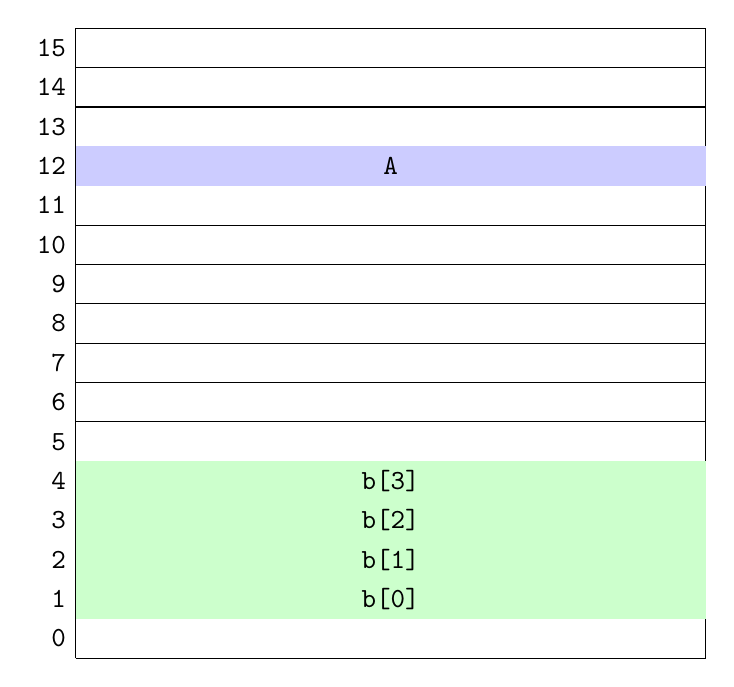
\begin{tikzpicture}
        \foreach \i in {0, 1, ..., 15} {
            \draw (0, \i*0.5) -- (8, \i*0.5); 
            \node[left] at (0, \i*0.5 + 0.25) {\texttt{\i}};
            \draw (0, \i*0.5) -- (0, \i*0.5 + 0.5); 
            \draw (8, \i*0.5) -- (8, \i*0.5 + 0.5);
        }

        \draw (0, 8) -- (8, 8);

        \foreach \i in {12} {
            \fill[blue!20] (0, \i*0.5) rectangle (8, \i*0.5 + 0.5);
        }
        \foreach \i in {1, 2, 3, 4 } {
            \fill[green!20] (0, \i*0.5) rectangle (8, \i*0.5 + 0.5);
        }
        \node at (4, 12*0.5 + 0.25) {\texttt{A}};
        \node at (4, 1*0.5 + 0.25) {\texttt{b[0]}};
        \node at (4, 2*0.5 + 0.25) {\texttt{b[1]}};
        \node at (4, 3*0.5 + 0.25) {\texttt{b[2]}};
        \node at (4, 4*0.5 + 0.25) {\texttt{b[3]}};
    \end{tikzpicture}
    }
    \caption{メモリアドレスとデータ}
    \vspace{-10pt}
    \subcaption{左側の数値はアドレスを表す}
    \vspace{-10pt}
    \subcaption{セル1つが1[byte]を表す}
    \end{figure}
    \end{column}
    \end{columns}
    \begin{textblock*}{0.3\linewidth}(300pt, 263pt)
        \hyperlink{63}{\beamerbutton{<}}
        \space
        \hyperlink{65}{\beamerbutton{>}}
    \end{textblock*}
\end{frame}

\section{ポインタ}
\begin{frame}[t, label=65]
    \frametitle{ポインタ}
    \tableofcontents[sections={2, 11}]
    \begin{textblock*}{0.3\linewidth}(300pt, 263pt)
        \hyperlink{64}{\beamerbutton{<}}
        \space
        \hyperlink{66}{\beamerbutton{>}}
    \end{textblock*}
\end{frame}

\subsection{ポインタの基本}
\begin{frame}[t, fragile, label=66]
    \frametitle{ポインタの基本}
    \begin{itemize}
        \item ポインタ\\
            変数のアドレスを値として格納できる変数をポインタという。
        \item ポインタの型\\
            ポインタには型があり、特定の型の変数を表すアドレスしか格納
            できない。
        \item ポインタの宣言\\
            変数名の前に*(ポインタ宣言子)をつければよい。
    \end{itemize}
    \begin{lstlisting}[gobble=8, caption=Example\space of\space Pointer\space Declaration]
        int *pint;
        double *px, *py;
        int i, *pi;
    \end{lstlisting}
    \begin{textblock*}{0.3\linewidth}(300pt, 263pt)
        \hyperlink{65}{\beamerbutton{<}}
        \space
        \hyperlink{67}{\beamerbutton{>}}
    \end{textblock*}
\end{frame}

\subsection{ポインタの初期化}
\begin{frame}[t, fragile, label=67]
    \frametitle{ポインタの初期化}
     ポインタとして宣言した変数にはアドレスを代入する。変数のアドレス
    は\verb|&|(アドレス演算子)を変数に作用させることで得る。
    \begin{lstlisting}[gobble=8, caption=Example\space of\space Pointer\space Initialization]
        int n, *np;
        double d, *dp;

        np = &n;
        dp = &d;
    \end{lstlisting}
     アドレスの値が気になるときはフォーマット指定子を\texttt{\%p}とし
    て表示させてみるとよいだろう。(16進数表記で出力される。)
    \begin{itembox}[l]{tips}
        \scalebox{2.4}{\textbf{ポインタには変数のアドレス}}\\
        が格納される。
    \end{itembox}
    \begin{textblock*}{0.3\linewidth}(300pt, 263pt)
        \hyperlink{66}{\beamerbutton{<}}
        \space
        \hyperlink{68}{\beamerbutton{>}}
    \end{textblock*}
\end{frame}

\subsection{ポインタによる間接アクセス}
\begin{frame}[t, fragile, label=68]
    \frametitle{ポインタによる間接アクセス}
     間接演算子*をポインタに作用させた式は、ポインタに格納された
    アドレスの指す値となる。(同じ記号を使うがポインタ宣言子とは名前が
    異なる)
    \begin{lstlisting}[gobble=8, caption=Pointer\space Example]
        int Var = 10;
        int *Ptr;

        Ptr = &Var;
        printf("Var=%d, *Ptr=%d", Var, *Ptr);

        *Ptr = 5;
        printf("Var=%d, *Ptr=%d", Var, *Ptr);
    \end{lstlisting}
    \begin{block}{出力}
        Var=10, *Ptr=10\\
        Var=5, *Ptr=5
    \end{block}
    \begin{textblock*}{0.3\linewidth}(300pt, 263pt)
        \hyperlink{67}{\beamerbutton{<}}
        \space
        \hyperlink{69}{\beamerbutton{>}}
    \end{textblock*}
\end{frame}

\subsection{図解}
\begin{frame}[c, fragile, label=69]
    \frametitle{図解}
    \framesubtitle{左側にコード、右側にその時のメモリ領域の図を示す。}
    \begin{columns}[c, totalwidth=0.98\linewidth]
    \begin{column}{.45\linewidth}
    \begin{lstlisting}[gobble=8]
        int Var = 10;
        int *Ptr;

        Ptr = &Var;
    \end{lstlisting}
     (右図でわかるように\texttt{*PtrとVarは等価であるため、*Ptrに対
    して値を代入することはVarに値を代入することと等しい。)}
    \end{column}
    \begin{column}{.50\linewidth}
    \begin{figure}
    \centering
    %\vspace{-20pt}
        \begin{tikzpicture}
              % Draw the variable box
              \node[draw, rectangle, minimum width=50pt, minimum height=25pt] (ptr) at (30, 40) {\texttt{0xbadc0ffeebad==}\verb|&|\texttt{Var}};

              % Draw the pointer box
              \node[draw, rectangle, minimum width=50pt, minimum height=25pt, above=50pt of ptr] (var) {\texttt{10}};

              % Draw arrow from pointer to variable
              \draw[->] (ptr.east) -- ++(10pt,0) -- node[right=-2pt]{\texttt{*Ptr(==Var)}}++(0, 75pt)-- (var.east);

              % Labels
              \node[above=3pt of var] {\texttt{Var}(変数)};
              \node[above=3pt of ptr] {\texttt{Ptr}(ポインタ)};
              \node[below=3pt of var] {\texttt{0xbadc0ffeebad}};
              \node[below=3pt of ptr] {\texttt{0xdeadbeefcafe}};
        \end{tikzpicture}
    \caption{ポインタとメモリ領域}
    \end{figure}
    \end{column}
    \end{columns}
    \begin{textblock*}{0.3\linewidth}(300pt, 263pt)
        \hyperlink{68}{\beamerbutton{<}}
        \space
        \hyperlink{70}{\beamerbutton{>}}
    \end{textblock*}
\end{frame}

\subsection{ポインタのポインタ}
\begin{frame}[t, fragile, label=70]
    \frametitle{ポインタのポインタ}
    \framesubtitle{みかん}
    %todo
    \begin{textblock*}{0.3\linewidth}(300pt, 263pt)
        \hyperlink{69}{\beamerbutton{<}}
        \space
        \hyperlink{71}{\beamerbutton{>}}
    \end{textblock*}
\end{frame}

\subsection{ポインタと配列}
\begin{frame}[t, fragile, label=71]
    \frametitle{ポインタと配列}
     配列名は配列の最初の要素を表すアドレスとなっている。
    つまり,\texttt{int a[10];}により配列を宣言した時、\texttt{a}と
    \verb|&|\texttt{a[0]は等価となる。このとき、aで初期化した
    ポインタに整数値nを足したポインタptr+nの値は、a[n]の
    アドレスと等価となる。}
    \begin{lstlisting}[gobble=8, caption=Exercise]
        int v[1000];
        int *ptr;

        ptr = v; // ptr = &v[0];

        for (int i = 0; i < 1000; i++) {
            printf("--------------------\n");
            printf("&v[%d]=\t%p\n", i, &v[i]);
            printf("ptr=\t\t%p\n", ptr);
            printf("v[%d]=\t\t%d\n", i, v[i]);
            printf("*ptr=\t\t%d\n", *ptr);
            ptr++;
        }
    \end{lstlisting}
    \begin{textblock*}{0.3\linewidth}(255pt, 130pt)
        \begin{itembox}[l]{出力の仕方}
             今回のように数千行を出力するときは、\texttt{./a.out > output}などとして実行し、ファイルに実行結果を出力するのが良い。
        \end{itembox}
    \end{textblock*}
    \begin{textblock*}{0.3\linewidth}(300pt, 263pt)
        \hyperlink{70}{\beamerbutton{<}}
        \space
        \hyperlink{72}{\beamerbutton{>}}
    \end{textblock*}
\end{frame}

\subsection{ポインタと関数}
\begin{frame}[c, fragile, label=72]
    \frametitle{ポインタと関数}
     ポインタを引数に取る関数を定義することができる。これにより、
    関数内で配列の値を参照できるようになる。(C言語では配列をそのまま引数
    とすることはできない)\\
     また、C言語の関数は返り値を1つしか持てないが、ポインタを使えば複数
    の値を返せる。
    \begin{textblock*}{0.3\linewidth}(300pt, 263pt)
        \hyperlink{71}{\beamerbutton{<}}
        \space
        \hyperlink{73}{\beamerbutton{>}}
    \end{textblock*}
\end{frame}
\end{document}
    \begin{lstlisting}[gobble=8, caption=example]
        double Norm(int, double *);
        
        int main(void)
        {
            double Vector[100];
            double *pvec, norm;

            for (int i = 0; i < 100; i++) {
                Vector[i] = i;
            }

            printf("norm=%e\n", Norm(100, Vector);
        }
    \end{lstlisting}

\subsection{}
\begin{frame}[t, fragile, label=73]
    \frametitle{サンプルコード}
    \begin{lstlistng}[gobble=8, caption=pra\_pointer\_1.c]
        #include<stdio.h>

        int main(void)
        {
            
        }
    \end{lstlisting}
    \begin{textblock*}{0.3\linewidth}(300pt, 263pt)
        \hyperlink{72}{\beamerbutton{<}}
        \space
        \hyperlink{74}{\beamerbutton{>}}
    \end{textblock*}
\end{frame}
